\documentclass{SHUarticle}
\title{\heiti{决策树分类算法总结}}
\date{\today}
\keyword{ID3\quad  C4.5\quad CART\quad  决策树减枝\quad 递归算法\quad }
\begin{document}
	\maketitle
	\begin{cnabstract}
		决策树是一种十分常见的分类和回归算法,决策树学习是从训练集中归纳出一种分类规则,并以树状图形的方式
		表现出来,可以看成为一个if-then规则的集合。决策树分类通常包含ID3、C4.5、CART三种算法,三者选择最优特征的方法有所不同:
		其中ID3算法使用的是信息增益;C4.5算法使用的是信息增益比;CART算法使用的是基尼指数。
		三种算法适用的场景也各不相同:
		\begin{itemize}
			\item ID3算法:适用于离散型数据。ID3算法使用信息增益来选择最佳的分裂变量,
			因此需要将数据集离散化为有限的分类。因此,
			ID3算法通常用于文本分类、垃圾邮件分类等离散型数据的分类问题。
			\item C4.5算法:适用于离散型和连续型数据。与ID3算法不同,
			C4.5算法使用信息增益比来选择最佳的分裂变量,能够处理连续型和离散型的数据,因此适用范围更广。另一方面:使用信息增益比来选择最佳划分特征,可以防止过度关注具有大量值的特征。C4.5算法常用于数据挖掘、信用评分等领域。
			\item  CART算法:适用于离散型和连续型数据,且CART算法可以用于分类与回归。该算法通过构建二叉树,来快速地进行分类和预测,
			因此该算法具有较高的准确性和鲁棒性,对于噪声数据和缺失值具有一定的容错性。
		\end{itemize}
		\par
		决策树很容易出现过拟合现象,即决策树很容易学习到训练集中所有的信息,
		这样一来,模型的泛化能力便会降低,因此为了减少决策树的过拟合现象,通常的手段有:{\heiti{预剪枝与后剪枝}}。其中预剪枝是在决策树的生成过程中便开始了,
		而后剪枝是要事先不加限制地生成一棵完整的决策树,然后自下而上地利用验证集进行剪枝。预剪枝在算法运行时间上上要少于后剪枝,但是针对不同的数据集,
		树允许的{\heiti{最大深度,叶节点所需的最小样本量}}需要自己进行调参;而后剪枝操作虽然训练成本增加,但是会提高模型的泛化能力。因此,选择预剪枝还是后剪枝操作取决于具体的数据集情况。
	\end{cnabstract}
	\tableofcontents %生成目录
	\newpage
\section{三种算法的优缺点}
\subsection{三种算法的优点}
\begin{itemize}
	\item ID3算法:算法简单易懂,计算效率高。
	对于数据缺失的情况有很好的处理能力。
	\item C4.5算法:
	\begin{itemize}
		\item 支持离散型和连续型数据的处理。
		\item  采用信息增益比来选择最佳分裂变量,能够避免ID3算法中选择取值较多的属性作为分裂变量的问题。
		\item 采用剪枝操作,能够有效地防止过拟合。
	\end{itemize}
	\item CART算法:
	\begin{itemize}
		\item 能够处理离散型和连续型数据的分类和回归问题。
		\item 采用基尼指数来选择最佳分裂变量,能够更好地处理连续型数据
		\item 采用剪枝操作,能够有效地防止过拟合.
	\end{itemize}
\end{itemize}
\subsection{三种算法的缺点}
\begin{itemize}
	\item ID3算法:
	\begin{itemize}
		\item 对于连续型数据的处理能力不足。
		\item 容易产生过拟合,不能很好地应对噪声数据。
	\end{itemize}
	\item C4.5算法:
	\begin{itemize}
		\item 对于噪声数据的处理能力不足。
		\item 计算效率较低,需要对数据进行多次扫描。
	\end{itemize}
	\item CART算法:
	\begin{itemize}
		\item CART算法生成的是二叉树,对于多分类问题需要进行二次划分,增加了计算复杂度。
		\item 对于缺失数据的处理能力有限。
	\end{itemize}
\end{itemize}
\section{算法数学原理}
\subsection{ID3算法}
ID3算法使用信息增益来选择数据的特征:样本D对特征A的信息增益:
\begin{equation}
	\begin{aligned}
	& g(D,A)=H(D)-H(D|A)\\
	&H(D) = -\sum\limits_{k=1}^K\frac{|c_k|}{|D|} \\ 
	&H(D|A)= \sum\limits_{i=1}^n\frac{|D_i|}{|D|}H(D_i) 
	\end{aligned}
	\end{equation}
利用ID3算法生成决策树的框架如下:
\begin{algorithm}
	\caption{Generate ID3 DecisionTree T }
	\label{algo:ref}
	\begin{algorithmic}[1]
		\REQUIRE X\_train,y\_train,feature\_names,depth=0.  % this command shows "Input"
		\ENSURE ~\\           % this command shows "Initialized"
		  确定预剪枝参数:max\_depth,min\_Samples\_split,min\_Samples\_leaf\\
		\WHILE {\emph{$X\_train$ $\neq \emptyset$ or $len(Counter(y\_train)$ $\neq 1 $)}}
		\STATE
		  1.计算X\_train的信息熵\\
		  2.如果y\_train中所有标签属于同一类$C_k$,则T为单结点树,将$C_k$作为类标记,返回T\\
		  3.如果X\_train = $\emptyset$,则T为单结点树,将y\_train中数量最大的类$C_k$作为该结点的类标记,返回T\\
		  4.按照(1)计算每个特征的信息增益,选择最优的特征$A_g$\\
		  5.特征$A_g$的每个取值$a_i$将D划分为多个非空子集$D_i$\\
		  6.遍历5中的$a_i$,令$X\_train$=$D_i$\textbf{递归}调用1-5,构建子树。
		\ENDWHILE
		\RETURN ID3 DecisionTree.  % this command shows "Output"
	\end{algorithmic}
\end{algorithm}

\subsection{C4.5算法}
C4.5算法使用的是信息增益比来选择数据的特征,样本D对特征A的信息增益
比为:
\begin{equation}
	\begin{aligned}
		& g_R(D,A) = \dfrac{g(D,A)}{H_A(D)}\\
		& H_A(D) = -\sum\limits_{i=1}^n \dfrac{|D_i|}{|D|}\log_2\frac{|D_i|}{|D|}
	\end{aligned}
\end{equation}
利用C4.5算法生成决策树的框架如下:
\begin{algorithm}
	\caption{Generate C4.5 DecisionTree T }
	\label{algo:ref}
	\begin{algorithmic}[1]
		\REQUIRE X\_train,y\_train,feature\_names,depth=0.  % this command shows "Input"
		\ENSURE ~\\           % this command shows "Initialized"
		  确定预剪枝参数:max\_depth,min\_Samples\_split,min\_Samples\_leaf\\
		\WHILE {\emph{$X\_train$ $\neq \emptyset$ or $len(Counter(y\_train)$ $\neq 1 $)}}
		\STATE
		  1.计算X\_train的信息熵\\
		  2.如果y\_train中所有标签属于同一类$C_k$,则T为单结点树,将$C_k$作为类标记,返回T\\
		  3.如果X\_train = $\emptyset$,则T为单结点树,将y\_train中数量最大的类$C_k$作为该结点的类标记,返回T\\
		  4.按照(2)计算每个特征的信息增益,选择最优的特征$A_g$\\
		  5.特征$A_g$的每个取值$a_i$将D划分为多个非空子集$D_i$\\
		  6.遍历5中的$a_i$,令$X\_train$=$D_i$\textbf{递归}调用1-5,构建子树。
		\ENDWHILE
		\RETURN C4.5 DecisionTree.  % this command shows "Output"
	\end{algorithmic}
\end{algorithm}
\section{CART分类算法}
\begin{definition}
	基尼指数:在分类问题中,假设有$K$个类,样本点
	属于第$k$类的概率为$p_k$,则概率分布的基尼指数为:
	\[Gini(p)=\sum\limits_{k=1}^Kp_k(1-p_k)\]
\end{definition}
特征A条件下集合D的基尼指数:
\[Gini(D,A)=\dfrac{|D_1|}{|D|}Gini(D_1)+\dfrac{|D_2|}{|D|}Gini(D_2)\]
CART算法构建的是二叉树模型,不仅要选择最优的特征进行分支,同时还
要选择最优特征的最优切分点
\section{决策树的剪枝}
决策树容易过拟合,因此我们需要对决策树进行剪枝操作,常见的减枝操作有预剪枝、后减枝。
\par 下面给一个对决策树进行预剪枝的示例:我们对make\_moons数据集分别建立两颗决策树,一颗不加限制,另一颗决策树要求叶节点
具有最小的样本数为4,否则不再继续向下分枝,对比两棵决策树的分类效果如下:
\begin{figure}[!h]
  \centering
  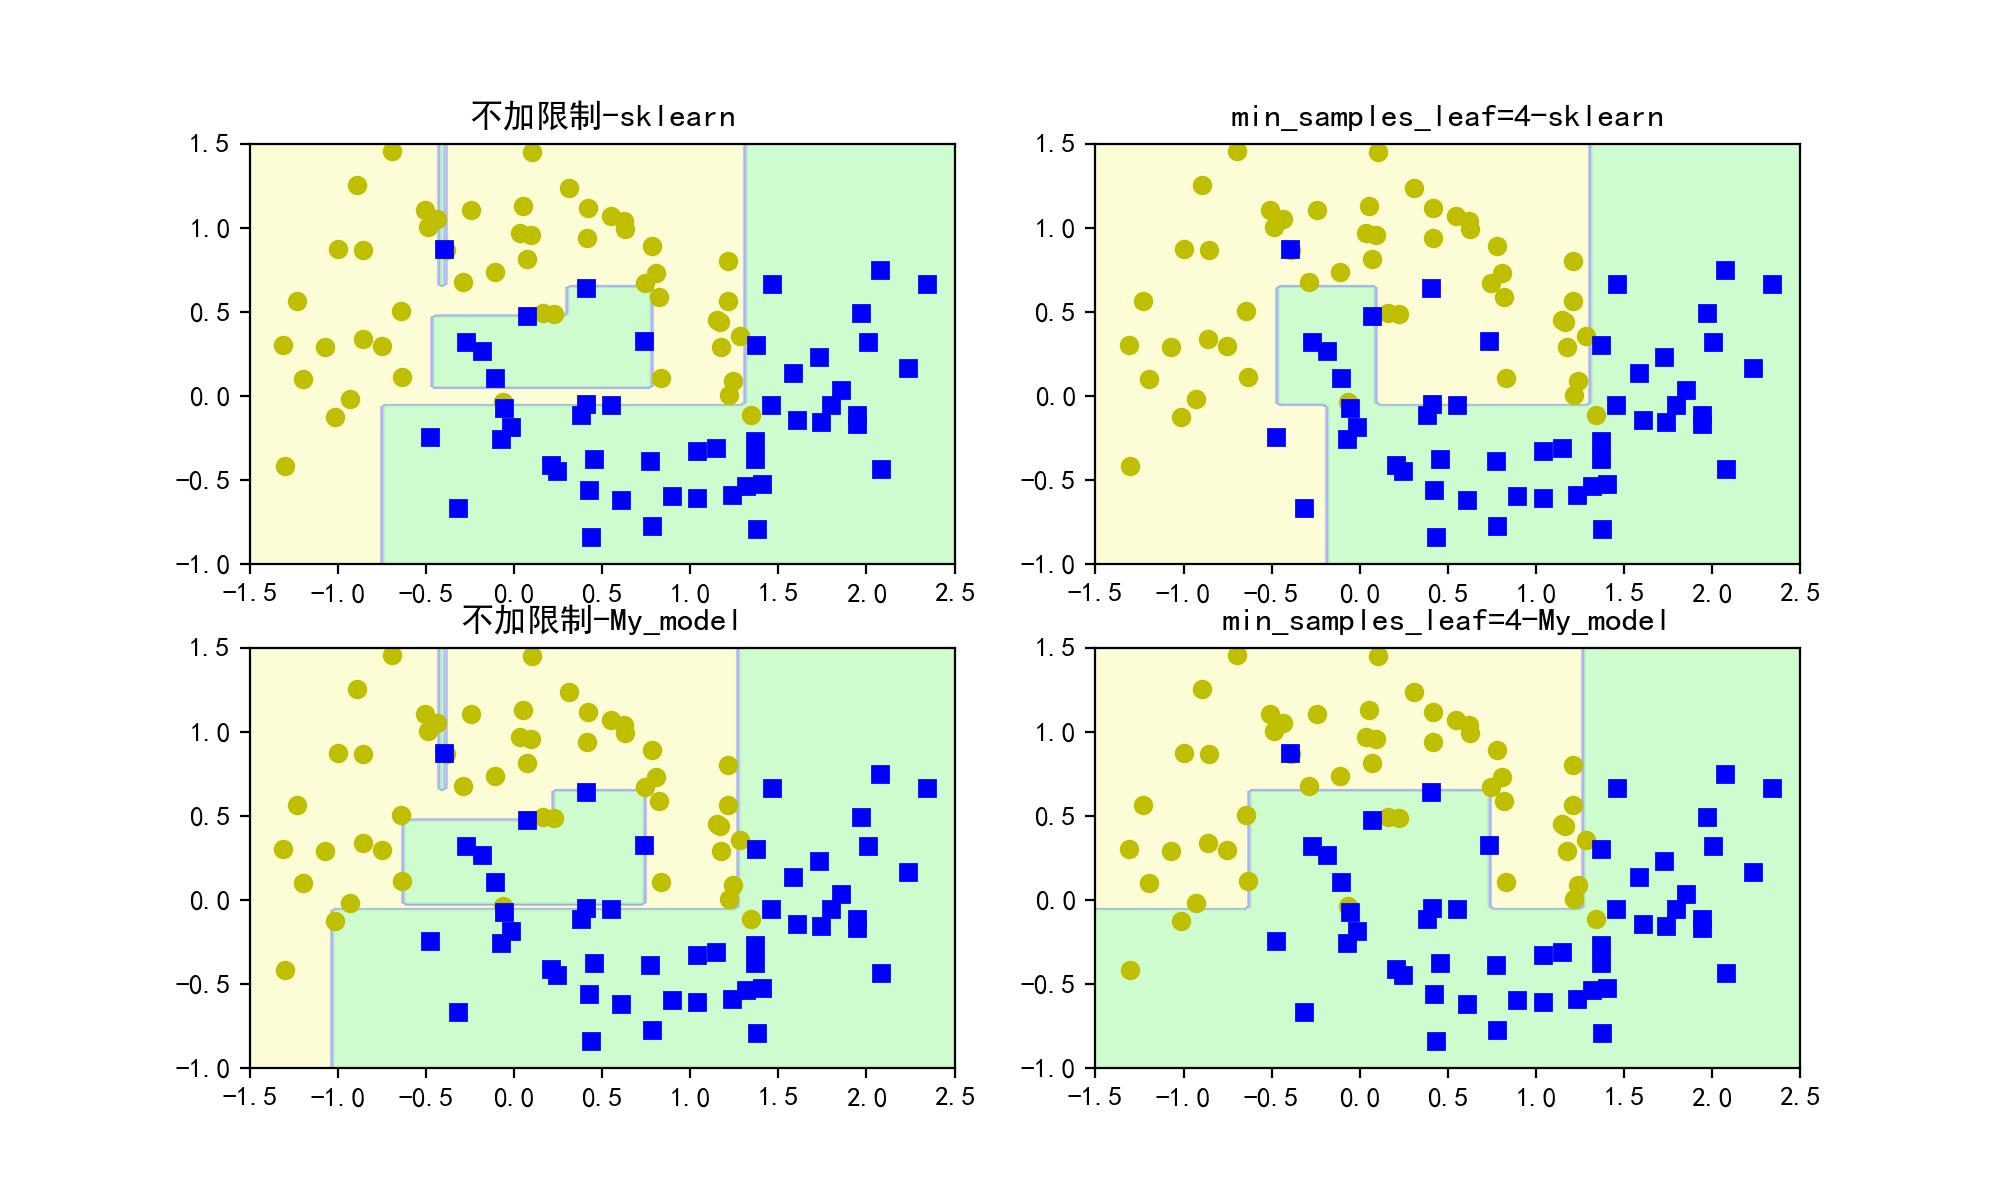
\includegraphics[scale = 0.6]{../Images/决策树预减枝.jpg}
  \caption{有无预剪枝的决策树边界对比}
  \label{fig:ex1}
\end{figure}
下面再给出一个决策树进行后剪枝的示例:同样的对make\_moons的数据集分别建立两颗决策树,其中一颗不加限制,第二棵进行后剪枝操作,
对比两棵决策树的分类效果如下:
\begin{figure}[!h]
	\centering
	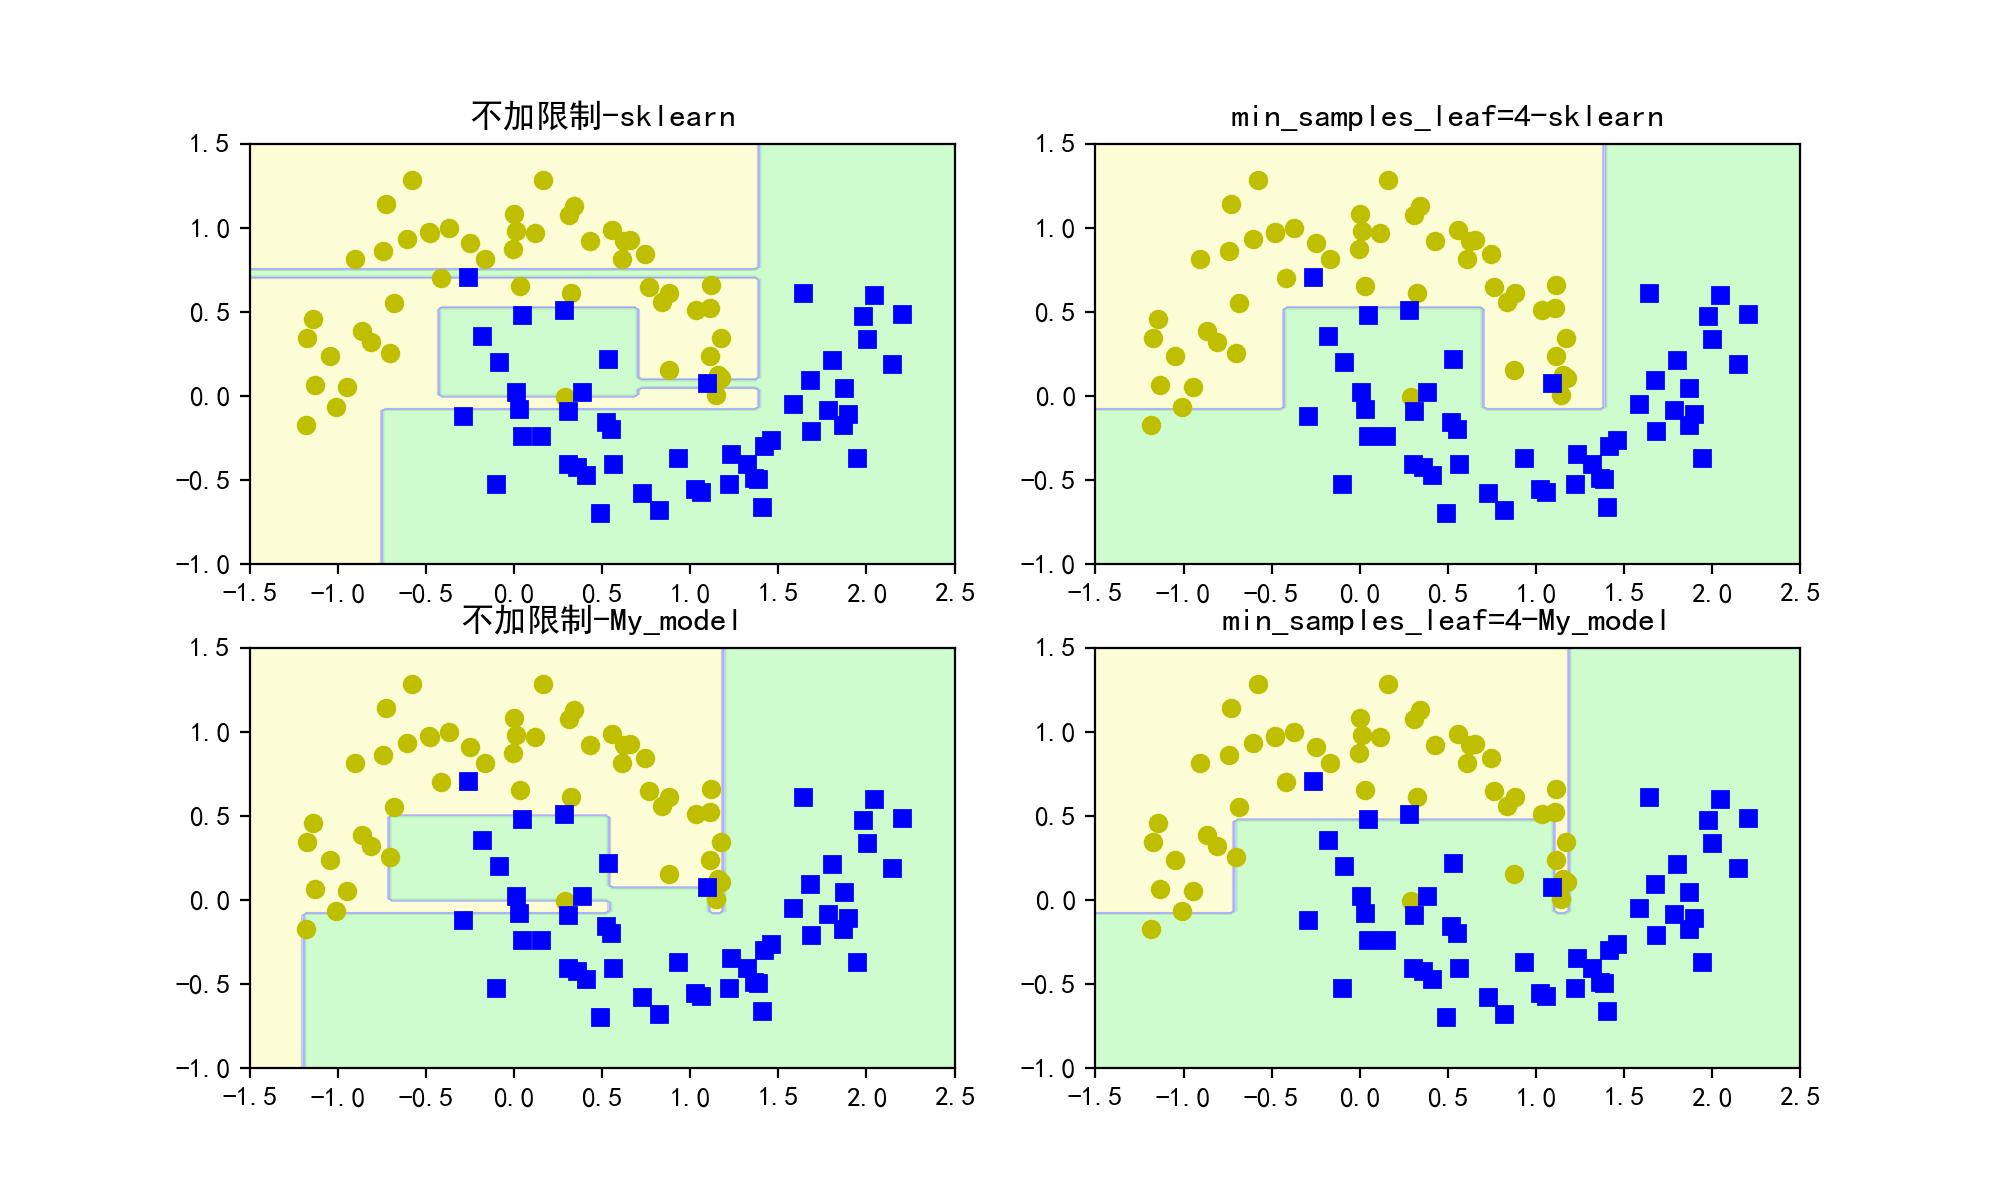
\includegraphics[scale=0.6]{../Images/决策树后剪枝.jpg}
	\caption{有无后剪枝的决策树边界对比}
	\label{fig2:ex2}
\end{figure}
从图\ref{fig:ex1}中可以看出:第一棵无剪枝决策树的边界十分复杂,很明显出现了过拟合
的现象.上面的两个子图是基于sklearn中的DecisionTreeClassifier函数的结果,下面的
两个子图是自己根据三种算法的数学原理自己编写的,可以看出,算法的复现是正确的。
\subsection{预剪枝}
一般来说,预剪枝对于何时停止决策树的生长有下面这几种方法:
1.当决策树达到一定的深度的时候,停止生长;
2.当到达当前节点的样本数量小于某个阈值的时候,停止树的生长;
3.计算决策树每一次分裂对验证集的准确度是否提升,当没有提升或者提升程度小于某个阈值的时候,则停止决策树的生长;
预剪枝具有思想直接、算法简单、效率高等特点,适合解决大规模的问题,但是如何准确地估计何时停止决策树的生长,针对不同的问题应该分别考虑,需要一定的经验判断。
\subsection{后剪枝}
决策树的预剪枝操作是在决策树生成的过程中就已经开始了,然而后剪枝操作是按照某种特征筛选准则
(ID3、C4.5、CART)先无限制地生成一颗决策树,然后在这棵决策树的
基础上进行自下而上的剪枝。\par 

决策树的后剪枝(post-pruning)是一种用于减小决策树过拟合的技术,
它通过修剪已经生成的决策树来提高模型的泛化能力。
后剪枝的过程是在决策树构建完成后进行的,具体步骤如下:
\begin{itemize}
	\item 将训练集分为训练集和验证集两部分,通常使用交叉验证的方法来得到验证集。
	\item 对于决策树的每个非叶节点,尝试将其替换成一个叶节点,并计算在验证集上的性能。
	\item 如果替换后的决策树在验证集上的性能没有降低,则接受替换操作,否则不接受替换操作,维持原来的决策树
	\item 重复步骤 2 和 3 直到所有非叶节点都被尝试过
\end{itemize}
需要注意的是,后剪枝过程可能会导致决策树的性能下降,因为我们可能会削减掉一些有用的分支.
因此,我们需要在训练集和验证集之间找到一个平衡点,以尽可能地减少过拟合的风险,同时保持模型的预测能力。
\end{document}